\ifx\wholebook\relax \else

\documentclass{article}
\usepackage[nomarginpar
  %, margin=.5in
]{geometry}

\addtolength{\oddsidemargin}{-0.05in}
\addtolength{\evensidemargin}{-0.05in}
\addtolength{\textwidth}{0.1in}

\usepackage[en]{../prelude}

\setcounter{page}{1}

\begin{document}

\title{Recursion}

\author{Liu Xinyu
\thanks{{\bfseries Liu Xinyu} \newline
  Email: liuxinyu95@gmail.com}}

\maketitle
\fi

\markboth{Recursion}{Mathematics of Programming}

\ifx\wholebook\relax
\chapter{Recursion}
\numberwithin{Exercise}{chapter}
\fi

\epigraph{GNU means \textbf{G}NU's \textbf{N}ot \textbf{Unix}}{--Richard Stallman}

\begin{wrapfigure}{R}{0.3\textwidth}
 \centering
 \includegraphics[scale=0.4]{img/Pythagoras.jpg}
 \captionsetup{labelformat=empty}
 \caption{Pythagoras (about 570BC - 490BC)}
 \label{fig:Pythagoras}
\end{wrapfigure}

People learn our world with numbers. In previous chapter, we introduced Peano axioms, and things that are isomorphic to natural numbers, like the list data structure in programming. Natural number is a fundamental tool, however, our building still need some corner stones. We accept the recursive definition without proof of its correctness, like the factorial for example.

\[
\begin{array}{l}
\textit{fact}(0) = 1 \\
\textit{fact}(n + 1) = (n + 1) \textit{fact}(n)
\end{array}
\]

Why does recursion work? What is the theory of recursion? Could we formally express recursion? We'll explore these questions in this chapter.

\section{Everything is number}

Pythagoras was the first mathematician and philosopher who studied the universe with numbers. He is famous all over the world in the theory named after him. He was born in the island of Samos, off the coast of modern Turkey. Pythagoras might have learnt from Thales of Miletus. With Thales suggestion, he went to oriental to learn about mathematics. He spent 13 years (22 years in other sayings) in Egypt. After the Persian Empire conquered Egypt, Pythagoras went eastward to Babylon with the army. He learned mathematics and astronomy from the Babylonians. Pythagoras might also arrive in India. Wherever he went, Pythagoras learned from the local scholars to enrich his knowledge. He did not only study hard, but also thought deeply. After long time of study, Pythagoras formed his own thoughts\cite{HanXueTao16}.

Pythagoras returned his hometown after long journey abroad and began to give lectures. Around 520BC, he left Samos, possibly because he disagreed with the local tyranny. He arrived in the Greek colony of Croton (southern Italy today). At Croton, he won trust and admiration of people, and founded the philosophical school of Pythagoreanism. Many prominent members of his school were women. The school was devoted to study astronomy, geometry, number theory, and music. They are called quadrivium, affected more than 2000 years of European education\cite{StepanovRose15}. Quadrivium reflects the Pythagoreans' philosophy, that everything is number. The planetary motion corresponds to geometry, while geometry is built on top of numbers. Numbers are also connected with music. The so-called Pythagoreans, who were the first to take up mathematics, not only advanced this subject, but saturated with it, they fancied that the principles of mathematics were the principles of all things. said Aristotle in Metaphysics. Pythagoras is the first one discovered the pattern of octave in mathematics. Pythagoras was revered as the founder of mathematics and music\footnote{There are different sayings about Pythagoras' death. His teachings of dedication and asceticism are credited with aiding in Croton's victory over the neighboring colony. After the victory, a democratic constitution was proposed, but the Pythagoreans rejected it. The supporters of democracy roused the populace against them. An attack was made upon them in some meeting-place. The building was set on fire, and many of the members perished; Different sources disagree regarding whether Pythagoras was killed, or if he managed to flee to Metapontum, where he lived out the rest of his life.}.

The Pythagoreans believed all things were made of numbers. They studied the numbers and the their connection to nature. They developed the early number theory, one of the most important area in mathematics. The pythagreans classified the natural numbers, defined many important concepts including even and odd numbers, prime and composite numbers and so on. They found some numbers equal to the sum of their proper postive divisors\footnote{The proer postive divisors are those positive divisors less than the number}, and named them as perfect numbers. For example 6 = 1 + 2 + 3, while 1, 2, 3 are the all three divisors of 6. Pythagoreans found the first two perfect numbers\footnote{Also known as complete numbers or ideal numbers. Euclid proved a formation rule (Euclid's Element, Book IX, proposition 35) whereby $q(q+1)/2$ is an even perfect number whenever $q$ is a prime of the form $2^p-1$ for prime $p$—what is now called a Mersenne prime. Much later, Euler proved that all even perfect numbers are of this form. This is known as the Euclid–Euler theorem.}. The smallest one is 6, the next is 28 (28 = 1 + 2 + 4 + 7 + 14). The Pythagorean also found a class of figurate numbers\footnote{The Pythagorean studied mathematics by making figures with small stones. The English word calculus comes from the Greek word stone\cite{HanXueTao16}.}, when they formed geometry figure with stones.

\begin{figure}[htbp]
%\begin{wrapfigure}{R}{0.4\textwidth}
\centering
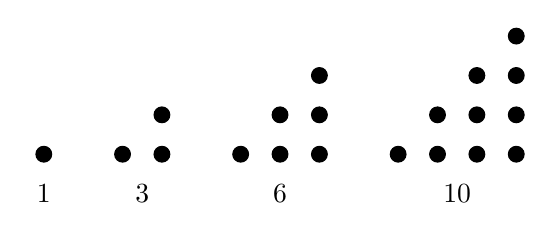
\begin{tikzpicture}[scale=0.5]
\filldraw (0, 0) circle (0.2);
\draw (0, -1) node{1};
\filldraw (2, 0) circle (0.2)
          (3, 0) circle (0.2)   (3, 1) circle (0.2);
\draw (2.5, -1) node{3};
\filldraw (5, 0) circle (0.2)
          (6, 0) circle (0.2)   (6, 1) circle (0.2)
          (7, 0) circle (0.2)   (7, 1) circle (0.2)   (7, 2) circle (0.2);
\draw (6, -1) node{6};
\filldraw (9, 0) circle (0.2)
          (10, 0) circle (0.2)    (10, 1) circle (0.2)
          (11, 0) circle (0.2)    (11, 1) circle (0.2)    (11, 2) circle (0.2)
          (12, 0) circle (0.2)    (12, 1) circle (0.2)    (12, 2) circle (0.2)    (12, 3) circle (0.2);
\draw (10.5, -1) node{10};
\end{tikzpicture}
\caption{Triangular number}
\label{fig:triangular-num}
%\end{wrapfigure}
\end{figure}

\begin{figure}[htbp]
%\begin{wrapfigure}{R}{0.4\textwidth}
\centering
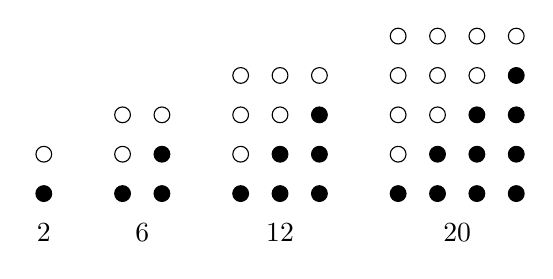
\begin{tikzpicture}[scale=0.5]
\draw (0, 1) circle (0.2);
\filldraw (0, 0) circle (0.2);
\draw (0, -1) node{2};

\draw (2, 1) circle (0.2)   (2, 2) circle (0.2)
      (3, 2) circle (0.2);
\filldraw (2, 0) circle (0.2)
          (3, 0) circle (0.2)   (3, 1) circle (0.2);
\draw (2.5, -1) node{6};

\draw (5, 1) circle (0.2)   (5, 2) circle (0.2)   (5, 3) circle (0.2)
      (6, 2) circle (0.2)   (6, 3) circle (0.2)
      (7, 3) circle (0.2);
\filldraw (5, 0) circle (0.2)
          (6, 0) circle (0.2)   (6, 1) circle (0.2)
          (7, 0) circle (0.2)   (7, 1) circle (0.2)   (7, 2) circle (0.2);
\draw (6, -1) node{12};

\draw (9, 1) circle (0.2)   (9, 2) circle (0.2)   (9, 3) circle (0.2)   (9, 4) circle (0.2)
      (10, 2) circle (0.2)   (10, 3) circle (0.2)   (10, 4) circle (0.2)
      (11, 3) circle (0.2)   (11, 4) circle (0.2)
      (12, 4) circle (0.2);
\filldraw (9, 0) circle (0.2)
          (10, 0) circle (0.2)    (10, 1) circle (0.2)
          (11, 0) circle (0.2)    (11, 1) circle (0.2)    (11, 2) circle (0.2)
          (12, 0) circle (0.2)    (12, 1) circle (0.2)    (12, 2) circle (0.2)    (12, 3) circle (0.2);
\draw (10.5, -1) node{20};
\end{tikzpicture}
\caption{Oblong number (number of rectangle)}
\label{fig:oblong-num}
%\end{wrapfigure}
\end{figure}

Figure \ref{fig:triangular-num} and \ref{fig:oblong-num} demonstrate the triangular numbers and oblong numbers (rectangle numbers). It's easy to figure out that the oblong number is two times of the corresponding triangle number. While the triangle number is the sum of the first $n$ postive integers. By this way, the Pythagoreans found the formula to calculate the sum of postive integers.

\[
1 + 2 + 3 + ... + n = \frac{1}{2}n(n+1)
\]

The Pythagoreans also found the odd number could be represented in gnomon\footnote{The word ``gnomon'' originally in Babylonia it probably meant and upright stick whose shadow was used to tell time. In Pythagoras' time it meant a carpenter's square. It also meant what was left over from a square when a smaller square was cut out of one corner. Later Euclid extended from square to parallelogram(\cite{MKlein1972}, p31).} shape as shown in figure \ref{fig:gnomon-num}. And the first $n$ gnomon shapes form a square, as in figure \ref{fig:square-num}. By this way, they found the formula to calculate the sum of $n$-odd numbers.

\[
1 + 3 + 5 + ... + (2n - 1) = n^2
\]

\begin{figure}[htbp]
%\begin{wrapfigure}{R}{0.4\textwidth}
\centering
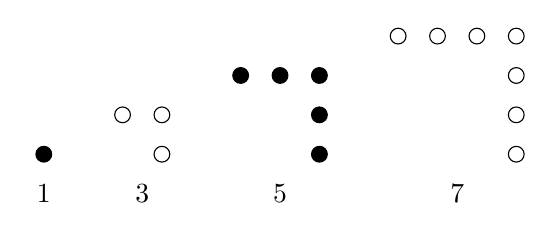
\begin{tikzpicture}[scale=0.5]
\filldraw (0, 0) circle (0.2);
\draw (0, -1) node{1};

\draw (2, 1) circle (0.2)
      (3, 0) circle (0.2)   (3, 1) circle (0.2);
\draw (2.5, -1) node{3};

\filldraw (5, 2) circle (0.2)   (6, 2) circle (0.2)   (7, 2) circle (0.2)
          (7, 0) circle (0.2)   (7, 1) circle (0.2);
\draw (6, -1) node{5};

\draw (9, 3) circle (0.2)   (10, 3) circle (0.2)   (11, 3) circle (0.2)   (12, 3) circle (0.2)
      (12, 0) circle (0.2)    (12, 1) circle (0.2)    (12, 2) circle (0.2);
\draw (10.5, -1) node{7};
\end{tikzpicture}
\caption{Gnomon number}
\label{fig:gnomon-num}
%\end{wrapfigure}
\end{figure}

\begin{figure}[htbp]
%\begin{wrapfigure}{R}{0.4\textwidth}
\centering
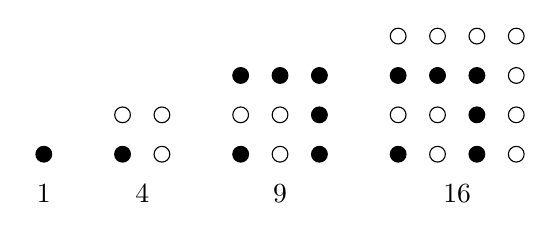
\begin{tikzpicture}[scale=0.5]
\filldraw (0, 0) circle (0.2);
\draw (0, -1) node{1};

\filldraw (2, 0) circle (0.2);
\draw (2, 1) circle (0.2)
      (3, 0) circle (0.2)   (3, 1) circle (0.2);
\draw (2.5, -1) node{4};

\filldraw (5, 0) circle (0.2);
\draw (5, 1) circle (0.2)
      (6, 0) circle (0.2)   (6, 1) circle (0.2);
\filldraw (5, 2) circle (0.2)   (6, 2) circle (0.2)   (7, 2) circle (0.2)
          (7, 0) circle (0.2)   (7, 1) circle (0.2);
\draw (6, -1) node{9};

\filldraw (9, 0) circle (0.2);
\draw (9, 1) circle (0.2)
      (10, 0) circle (0.2)   (10, 1) circle (0.2);
\filldraw (9, 2) circle (0.2)   (10, 2) circle (0.2)   (11, 2) circle (0.2)
          (11, 0) circle (0.2)   (11, 1) circle (0.2);
\draw (9, 3) circle (0.2)   (10, 3) circle (0.2)   (11, 3) circle (0.2)   (12, 3) circle (0.2)
      (12, 0) circle (0.2)    (12, 1) circle (0.2)    (12, 2) circle (0.2);
\draw (10.5, -1) node{16};
\end{tikzpicture}
\caption{Square number and gnomon numbers}
\label{fig:square-num}
%\end{wrapfigure}
\end{figure}

This is the answer to the exercise problem in chapter 1. With these facts, the Pythagoreans found there were many things could be explained in numbers. Given two strings under the same tension, it's said Pythagras found the tune was harmonic if the ratio of their lengths is an integer. He developed the earlist music theory based on this. It seemed that music and mathematics were totally different things, while finally Pythagoras concluded that music was mathematics. Such unexpected relationship impacted Pythagoras greatly. He guessed that all things could be explained with integers or the ratio of integers. The Pythagoreans started to find more and more things connected to nunbers, they believed the meaning of the whole universe was the harmonic of numbers, and developed the phylosophy based on number. This led to the attempt to build the geometry also on top of the numbers, so the overall mathematics is based on integers.

The Pythagoreans' most famous achievement is the Pythagoras theorem. However, we'll see later, this theorem is a double-edged sward. It led to a recursive circle, and revealed the loophole of the idea that everything is number. In order to understand this, we need introduce the concept of commensurable and the Euclidean algorithm. To build the geometry on top of the numbers, The Pythagoreans defined how to measure a line segment with another, if segment A can be represented by duplicating segment V finite times, we say V measures A. It means the length of one segment is the integer times of the other. There can be varies of measurements for a given line. When one can use the same segment to measure different lines, it has to be the common measure. That is to say if and only if segment V can measure both A and B, it is the common measure of them. The Pythagoreans believed for any two segments, there must be a common measure. If this was true, then the whole geometry can be built on top of numbers.

%\begin{wrapfigure}{R}{0.4\textwidth}
\begin{figure}[htbp]
 \centering
 \includegraphics[scale=0.2]{img/Pythagoras-proof.png}
 \caption{One of the methods to prove the Pythagoras theorem. The areas in white are same.}
 \label{fig:Pythagoras-proof}
\end{figure}
%\end{wrapfigure}

\section{The Euclidean algorithm}

As there can be mutliple common measures, we define the biggest one as the greatest common measure. Formally speaking, if segment V is the common measure of A and B, and V is greater than any other common measures, we say V is the greatest common measure of A and B. Given two segments, how to find the greatest common measure? There is a famous acient recursive method, called the Euclidean algorithm can solve this problem. It is named after the great ancient Greek methematician Euclid\footnote{The Euclidean algorithm was also developed independently in ancient India and China. The Indian mathematician Aryabhata used this method to solve the Diophantine equation around the end of the 5th centry. The Euclidean algorithm was treated as a special case of the Chinese remainder theorem in {\em Sunzi Suanjing}. Qin Jiushao gave the detailed algorithm in his {\em Mathematical Treatise in Nine Sections} (数书九章) in 1247.}. This algorithm is defined as proposition 3, in book X\footnote{The same algorithm for integers is also defined as propostion 1, book VII. However, the algorithm for segements covers the integer case.} of Euclid's Elements\cite{Elements}.

\subsection{The Euclid's Elements}

\begin{wrapfigure}{R}{0.35\textwidth}
%\begin{figure}[htbp]
 \centering
 \includegraphics[scale=0.65]{img/Euclid.jpg}
 \captionsetup{labelformat=empty}
 \caption{Euclid, About 300BC}
 \label{fig:Euclid}
%\end{figure}
\end{wrapfigure}

Euclid of Alexandria is the most prominent ancient Greek mathematician, often referred as ``father of geometry''. His {\em Elements} is one of the most influential works in the history. However, little is known of Euclid's life except that he taught at Alexandria in Egypt. The year and place of his birth and death are unknown. Proclus, the last major Greek philosopher who lived around 450AD introduced Euclid briefly in his {\em Commentary on the Elements}. He mentioned an interesting story about Euclid. When Ptolemy I of Alexandria (king of Egypt 323BC - 283BC) grew frustrated at the degree of effort required to master geometry via Eculid's {\em Elements}, he asked if there was a shorter path, Euclid replied there is no royal road to geometry. This becomes the learning maxim of eternal. Another story told by Stobaeus said someone who had begun to learn geometry with Euclid, when he had learnt the first theorem, asked Euclid ``What shall I get by learning these things?'' Euclid said ``Give him three pence since he must make gain out of what he learns''. Euclid disagreed with the narrow practical view of learning\cite{Elements}.

From ancient time to the late 19th century, people considered the {\em Elements} as a perfect example of correct reasoning. Although many of the results in {\em Elements} originated with earlier mathematicians, one of Euclid's accomplishments was to present them in a single, logically coherent framework, making it easy to use and easy to reference, including a system of rigorous mathematical proofs that remains the basis of mathematics 23 centuries later. More than a thousand editions have been published, making it one of the most popular books after the Bible. Even today, {\em Elements} is still widely taught in school\footnote{The most popular version is edited by the French mathematician Lagrange (1736 - 1813).} as one of the basic way to train logic reasoning\cite{HanXueTao16}.

\subsection{Euclidean algorithm}

\begin{proposition}[Euclid's Elements, Book X, Proposition 3]
To find the greatest common measure of two given commensurable magnitudes.
\end{proposition}

The solution Euclid gave only uses recursion and subtraction. It means the greatest common measure can be solved only with ruler and compass essentially. This algorithm can be formalized as the following\footnote{Term `gcm' is the abbreviation for the greatest common measure. When $a$ and $b$ are integers, we often use `gcd' as the abbreviation for the greatest common divisor.}.

\be
\gcm(a, b) = \left \{
  \begin{array}
  {r@{\quad:\quad}l}
  a = b & a \\
  b < a & \gcm(a - b, b) \\
  a < b & \gcm(a, b - a)
  \end{array}
\right.
\label{eq:gcm-minus}
\ee

Suppose segement $a$ and $b$ are comensurable. If they are equal, then either one is the greatest common measure, we can return $a$ as the result. If $a$ is longer than $b$, we can use compass to intercept $b$ from $a$ repeatedly (through recursion), then find the greatest common measure for the intercepted segment $a'$ and $b$; otherwise if $b$ is longer than $a$, we intercept $a$ from $b$ repeatedly, and find the greatest common measure for the segment $a$ and $b'$. Figure \ref{fig:line-seg-gcm} illustrated the steps when processing two segments. We can also use this algorithm to process two integers 42 and 30. The detailed steps are list in the following table.

\begin{figure}[htbp]
\centering
\begin{tikzpicture}[scale=0.15]

\filldraw (0, 0) circle (0.5)   (30, 0) circle (0.5)   (42, 0) circle (0.5);
\draw (-8, 0) node{$a$} (0, 0) -- (42, 0);
\filldraw (0, -5) circle (0.5)   (30, -5) circle (0.5);
\draw (-8, -5) node{$b$} (0, -5) -- (30, -5);

\filldraw (0,  -15) circle (0.5)   (12, -15) circle (0.5);
\draw (-8, -15) node{$a'=a-b$} (0, -15) -- (12, -15);
\filldraw (0, -20) circle (0.5)   (12, -20) circle (0.5)   (24, -20) circle (0.5)   (30, -20) circle (0.5);
\draw (-8, -20) node{$b$} (0, -20) -- (30, -20);

\filldraw (0,  -30) circle (0.5)   (6, -30) circle (0.5)   (12, -30) circle (0.5);
\draw (-8, -30) node{$a'$} (0, -30) -- (12, -30);
\filldraw (0, -35) circle (0.5)   (6, -35) circle (0.5);
\draw (-8, -35) node{$b'=b-2a'$} (0, -35) -- (6, -35);

\filldraw (0,  -45) circle (0.5)   (6, -45) circle (0.5);
\draw (-8, -45) node{$a''=a'-b'$} (0, -45) -- (6, -45);
\filldraw (0, -50) circle (0.5)   (6, -50) circle (0.5);
\draw (-8, -50) node{$b'$} (0, -50) -- (6, -50);

\end{tikzpicture}
\caption{Euclidean algorithm example steps.}
\label{fig:line-seg-gcm}
\end{figure}

\vspace{5mm}

\begin{tabular}{|l|l|l|}
\hline
$\gcm(a, b)$ & $a$ & $b$ \\
\hhline{|=|=|=|}
$\gcm(42, 30)$ & 42 & 30 \\
\hline
$\gcm(12, 30)$ & 12 & 30 \\
\hline
$\gcm(12, 18)$ & 12 & 18 \\
\hline
$\gcm(12, 6)$ & 12 & 6 \\
\hline
$\gcm(6, 6)$ & 6 & 6 \\
\hline
\end{tabular}

\vspace{5mm}

Repeatedly subtracting $b$ from $a$ to get $a'$, it's exactly the definition of division with remainder: $a' = a - \lfloor a / b \rfloor b$, or denoted as $a'= a \bmod b$. We can use the division with remainder to replace the repeated subtraction in the origin Euclidean algorithm. Besides that, when one magnitude is an integer multiple of the other, for example $b \leq a$ and $a$ can be divided by $b$, we know the greatest common measure is $b$. As the remainder $a \bmod b = 0$, we define $\gcm(0, b) = \gcm(b, 0) = b$. We can compare $a$ and $b$ first, then exchange them if $a < b$. As we know $a \bmod b$ must be less than $b$, when recursively compute the next time, we can directly exchange them as $\gcm(b, a \bmod b)$. This gives the improved Euclidean algorithm.

\be
\gcm(a, b) = \left \{
  \begin{array}
  {r@{\quad:\quad}l}
  b = 0 & a\\
  \text{otherwise} & \gcm(b, a \bmod b) \\
  \end{array}
\right.
\label{eq:gcm}
\ee

Why does this algorithm give the greatest common measure? We prove it with two steps. At step one, we prove this algorithm gives the common measure. Suppose $b \leq a$, let the integer $q_0$ be the quotient, $r_0$ be the remainder. We have $a = b q_0 + r_0$. As we get the common measure if $r_0$ is zero, let's focus on the case that $r_0$ is not zero. We can next express $b$ as $b = r_0 q_1 + r_1$, and list the similar equations unless the remainder is not zero.

\[
\begin{array}{rcl}
a &=& b q_0 + r_0 \\
b &=& r_0 q_1 + r_1 \\
r_0 &=& r_1 q_2 + r_2 \\
r_1 &=& r_2 q_3 + r_3 \\
& & ...
\end{array}
\]

This list grows as long as $a$ and $b$ are commensurable. But it is not infinite. This is because every time, we use compass to intercept integer times. The quotients are integers. And all the remainders are less than the relative divisors. We have $b > r_0 > r_1 > r_2 > ... > 0$. As the remainder can not be less than zero, and the initial magnitude is finite, we must reach to $r_{n-2} = r_{n-1} q_n$ within finite steps.

Next is to prove $r_{n-1}$ can measure both $a$ and $b$. Obviously $r_{n-1}$ measures $r_{n-2}$ by definition. Consider the last second equation $r_{n-3} = r_{n-2} q_{n-1} + r_{n-1}$, since $r_{n-1}$ measures $r_{n-2}$, $r_{n-1}$ also measures $r_{n-2} q_{n-1}$. So it measures $r_{n-2} q_{n-1} + r_{n-1}$, which equals to $r_{n-3}$. Similiarily, we can prove $r_{n-1}$ measures the left hand of every equations step by step upwards to $b$ and $a$. Thus proves the answer found by Euclidean algorithm, $r_{n-1}$ is the common measure of $a$ and $b$. Suppose the greatest common measure is $g$, we have $r_{n-1} \leq g$.

The next step is to prove, for any common measure $c$ for $a$ and $b$, it measures $r_{n-1}$. As $c$ is the common measure, both $a$ and $b$ can be expressed with it, let $a = mc$, $b = nc$, where $m$ and $n$ are some integers. Then the first equation $a = b q_0 + r_0$ can be denoted as $mc = ncq_0 + r_0$, as we know $r_0 = (m - nq_0)c$, it means $c$ measures $r_0$. Similarily, we can prove $c$ measures $r_1$, $r_2$, ..., $r_{n-1}$ one by one. Thus we proved any common measure also measures $r_{n-1}$, so the greatest one $g$ also measures $r_{n-1}$. It means $g \leq r_{n-1}$.

Combine the results from step one and two, that $r_{n-1} \leq g$ and $g \leq r_{n-1}$, we deduce the greatest common measure $g = r_{n-1}$. It does not only prove the correctness of Euclidean algorithm, but also tells us $g$ is the greatest common measure for every pair of magnitudes:

\be
g = \gcm(a, b) = \gcm(b, r_0) = ... = \gcm(r_{n-2}, r_{n-1}) = r_{n-1}
\label{eq:recursive-gcm}
\ee

\begin{figure}[htbp]
 \centering
 \subcaptionbox{Recursively cut off squares}{\includegraphics[scale=0.45]{img/GCM.png}}
 \subcaptionbox{Tile the small squares}{
   \begin{adjustbox}{max width=\textwidth}
   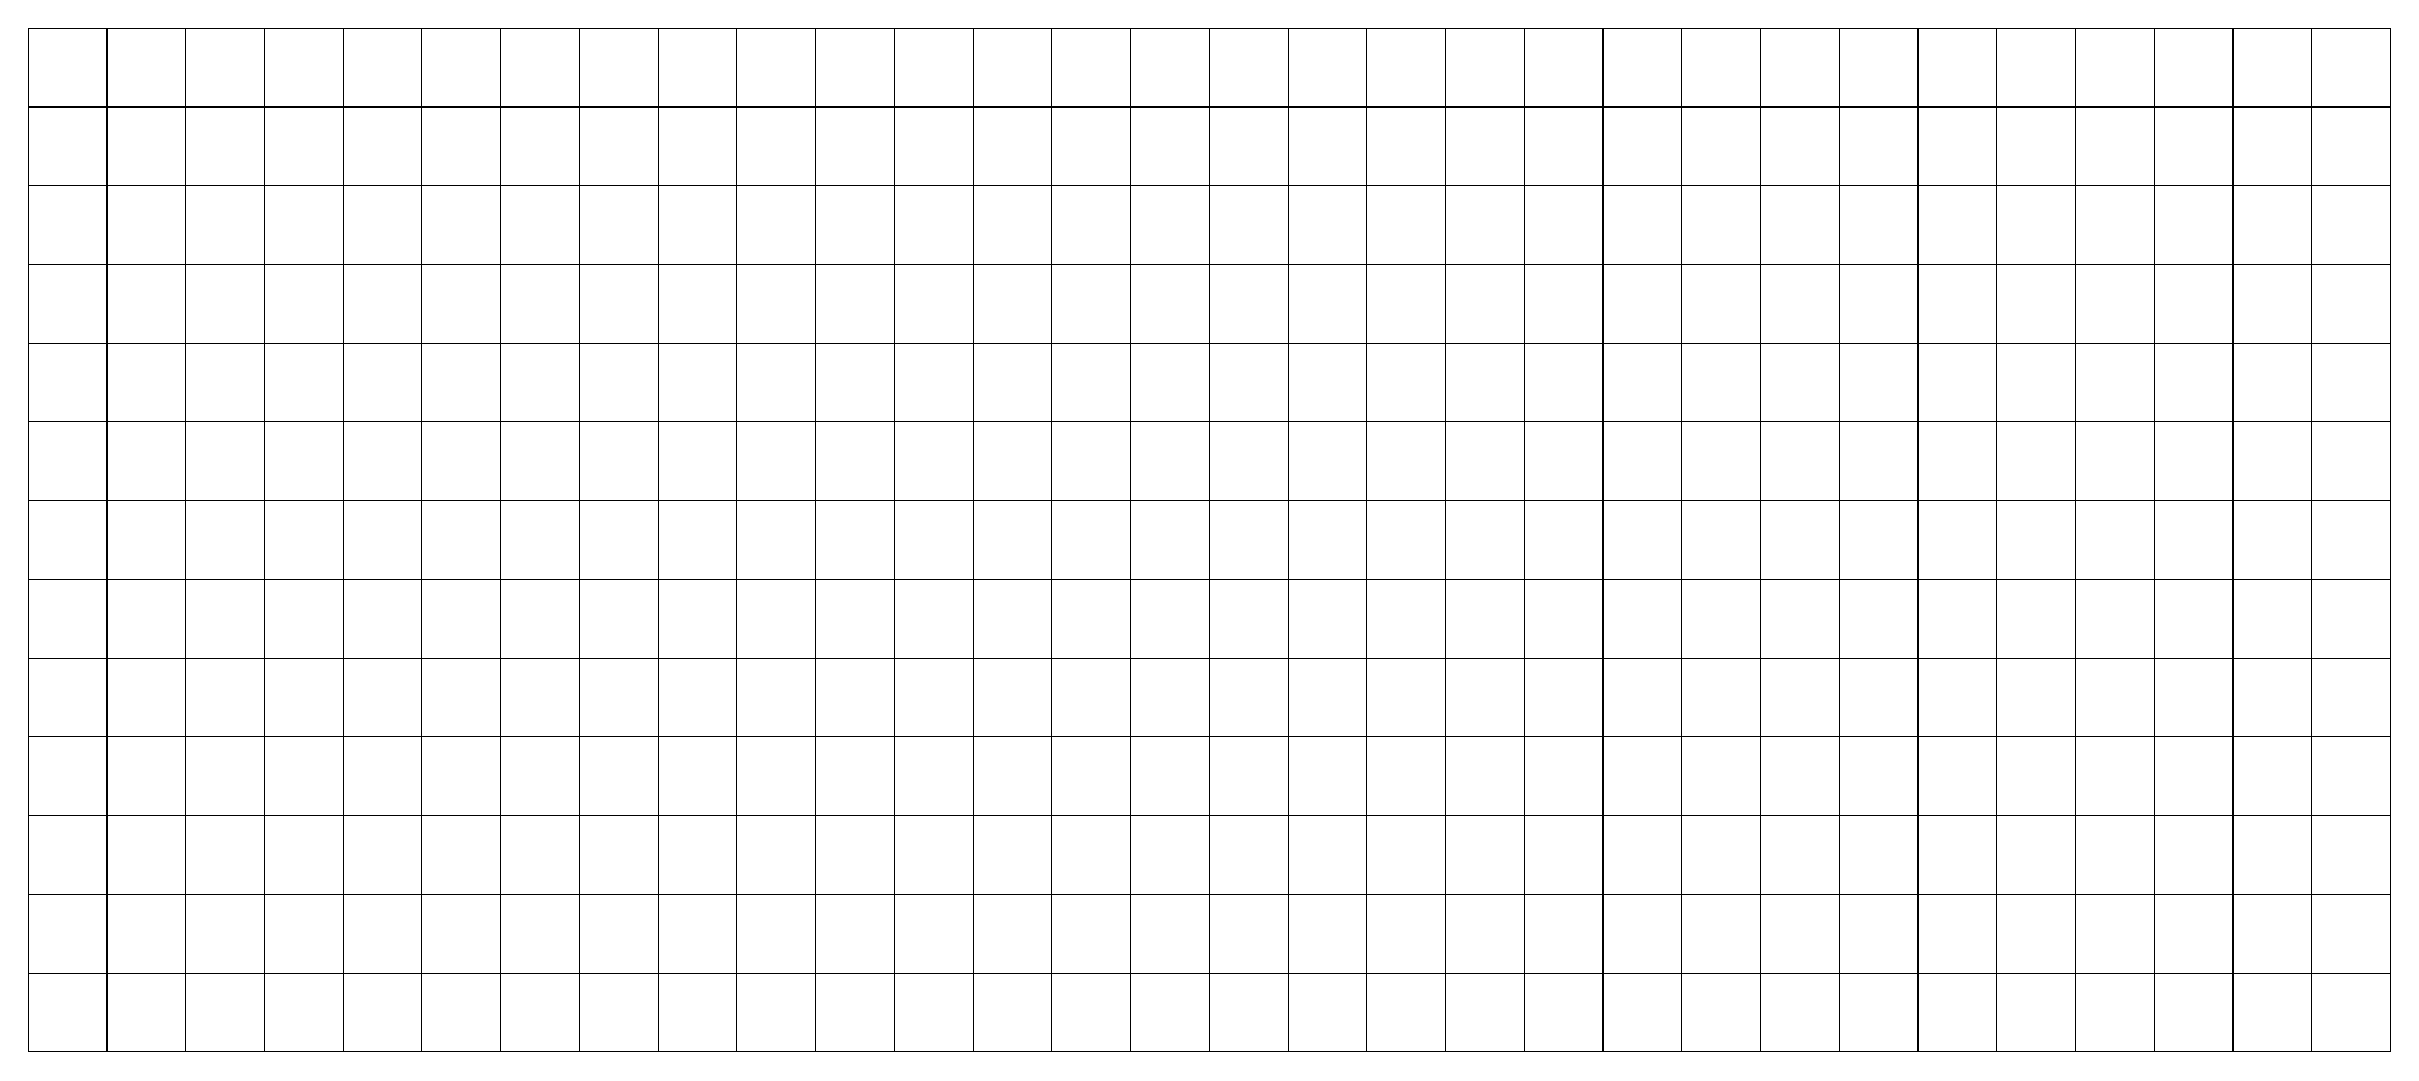
\begin{tikzpicture}
     \draw[step=1, thin] (0, 0) grid (30, 13);
   \end{tikzpicture}
   \end{adjustbox}
 }
 \captionsetup{labelformat=empty}
 \caption{A geometric description of Euclidean algorithm}
 \label{fig:geometric-GCM}
\end{figure}

\subsection{Extended Euclidean algorithm}

The extended Euclidean algorithm is an extension to the Euclidean algorithm. For given magnitude $a$ and $b$, in addition to compute their greatest common measure $g$, it can also find two integers $x$ and $y$, that satisfy Bézout's identity $ax + by = g$. Why does Bézout's identity\footnote{Bézout's identity, or Bézout's theorem was first found and proven by French mathematician Méziriac (Claude Gaspard Bachet de Méziriac,1581–1638) for integers. Bézout proved it hold for polynomials. Bézout identity can be extended to any Euclidean domain and Principle Idean Domain (PID).} always hold? Here is a proof. We can construct a set, consists of all the positive linear combinations of $a$ and $b$.

\[
S = \{ ax + by | x, y \in \mathbb{Z}\ \text{and} \ ax + by > 0\}
\]

%\begin{wrapfigure}{R}{0.4\textwidth}
\begin{figure}[htbp]
 \centering
 \subcaptionbox{Étienne Bézout, 1730 - 1783}[0.45\linewidth]{\includegraphics[scale=0.45]{img/Bezout.jpeg}}
 \subcaptionbox{Claude Gaspard Bachet de Méziriac, 1581–1638, who first discovered and proved Bézout's idendity for integers.}[0.45\linewidth]{\includegraphics[scale=0.95]{img/Meziriac.jpg}}
 \captionsetup{labelformat=empty}
 \caption{}
 \label{fig:Bezout}
 \label{fig:Meziriac}
\end{figure}
%\end{wrapfigure}

For line segments, $S$ must not be empty, as it contains at least $a$ (where $x = 1, y = 0$) and $b$ (where $x = 0, y = 1$). Since all the elements in $S$ are positive, there must exist the smallest one. We denote the smallest element as $g = as + bt$. We'll next show that $g$ is the greatest common measure of $a$ and $b$. Let's express $a$ as the quotient and remainder of $g$.

\be
a = qg + r
\label{eq:Euclidean-division}
\ee

Where the remainder $0 \leq r < g$. It is either zero or belongs to set $S$, this is because:

\[
\begin{array}{rll}
r & = a - qg & \text{From (\ref{eq:Euclidean-division})} \\
  & = a - q(as + bt) & \text{Definition of}\ g \\
  & = a(1 - qs) - bqt & \text{Change to combination of}\ a\ \text{and}\ b
\end{array}
\]

It means $r$ can be expressed as the linear combination of $a$ and $b$, therefore, if it's not zero, it must belong to set $S$. However, this is not possible because we previously defined $g$ as the least postive element in $S$, while $r$ is less than $g$. To avoid this contradition, we know that $r$ has to be zero. From equation (\ref{eq:Euclidean-division}), $g$ measures $a$. With the same method, we can prove $g$ also measures $b$. Therefore $g$ is the common measure of them. We'll next prove that $g$ is the greatest one. Consider an arbitrary common measure $c$ for $a$ and $b$, according to the definition, there exists integers $m$ and $n$, that $a = mc$ and $b = nc$. Then $g$ can be expressed as:

\[
\begin{array}{rll}
g & = as + bt & \text{The definition} \\
  & = mcs + nct & \text{$c$ is common measure of $a$ and $b$} \\
  & = c(ms + nt) & \text{$g$ is multiple of $c$}
\end{array}
\]

It means $c$ measure $g$, so $c \leq g$. It gives that $g$ is the greatest common measure. Summarize the above, we complete the proof of Bézout's identity. There exists integers, that $ax + by = g$ holds. Besides that, we know the greatest common measure is the minimum postive values among all the linear combinations.

We can deduce the extended Euclid algorithm with Bézout's idendity.

\[
\begin{array}{rlr}
ax + by & = \gcm(a, b) & \text{Bézout's idendity} \\
        & = \gcm(b, r_0) & \text{Euclid algorithm (\ref{eq:recursive-gcm})} \\
        & = bx' + r_0 y' & \text{Use Bézout's idendity for $b$ and $r_0$} \\
        & = bx' + (a - bq_0)y' & \text{By $a = b q_0 + r_0$} \\
        & = ay' + b(x' - y'q_0) & \text{As linear combination of $a$ and $b$} \\
        & = ay' + b(x' - y' \lfloor a / b \rfloor) & \text{$q_0$ as the quotient of $a$ and $b$}
\end{array}
\]

This gives the recursive case:

\[
\left \{
  \begin{array}{l}
  x = y' \\
  y = x' - y' \lfloor a / b \rfloor
  \end{array}
\right.
\]

The edge case happens when $b = 0$, we have $\gcm(a, 0) = 1a + 0b$. Combine it with the recursive case, we obtain the extended Euclidean algorithm.

\be
\gcm_{ex}(a, b) = \left \{
  \begin{array}
  {r@{\quad:\quad}l}
  b = 0 & (a, 1, 0) \\
  \text{otherwise} & \begin{array}{l}
                (g, y', x' - y' \lfloor a / b \rfloor) \\[2pt]
                \text{其中}(g, x', y') = \gcm_{ex}(b, a \bmod b)
                \end{array} \\
  \end{array}
\right.
\label{eq:gcm-ext}
\ee

Here is a puzzle can be solved with the extended Euclidean algorithm(\cite{LiuXinyu2017}, p50). Given two jars with capacity of 9 and 4 gallons, how to get 4 gallons of water from the river?

There are some variances of this puzzle. The capacities can be other nunmbers. It's said the French mathematician Sim\`{e}on Denis Poisson solved this puzzle when he was a child.

There are total six operations between two jars. Denote the big one as $A$ with capacity of $a$; denote the small one as $B$ with capacity of $b$:

\begin{itemize}
\item Fill the big jar $A$;
\item Fill the small jar $B$;
\item Empty the big jar $A$;
\item Empty the small jar $B$;
\item Pour the water from jar $A$ to jar $B$;
\item Pour the warer from jar $B$ to jar $A$.
\end{itemize}

The last two operations stop when either jar is empty or full. Below example shows a list of operations (suppose $b < a < 2b$ hold).

\begin{table}[htbp]
\centering
\begin{tabular}{l|l|l}
$A$ & $B$ & Operation \\
\hline
0 & 0 & start \\
0 & b & fill $B$ \\
b & 0 & pour from $B$ to $A$ \\
b & b & fill $B$ \\
a & 2b - a & pour from $B$ to $A$ \\
0 & 2b - a & empty $A$ \\
2b - a & 0 & pour from $B$ to $A$ \\
2b - a & b & fill $B$ \\
a & 3b - 2a & pour from $B$ to $A$ \\
... & ... & ... \\
\end{tabular}
\caption{The water in the jars and the operations.} \label{tab:jug-ops}
\end{table}

No matter what sequence of operations, the water in the jars can always be expressed as $ax + by$ where $x$ and $y$ are integers. It means the water we get is the linear combination of $a$ and $b$. From the proof of Bézout's identity, we know the smallest positive number of this linear combination is exactly the greatest common measure $g$. We can tell if it is possible to get $c$ gallons of water if and only if $c$ can be measured by $g$\footnote{If and only if $c$ can be devided by the greatest common divisor $g$ for integer capacities.}. We assume $c$ is not greater than the capacity of the bigger jar.

For example, we can't get 5 gallons of water with two jars of 4 gallons and 6 gallons. This is because the greatest common divisor of 4 and 6 is 2. Which can't divide 5. (In other words, we can't get odd galons of water with two jars of even gallons capacities.) If $a$ and $b$ are coprime, i.e. $\gcd(a, b) = 1$, then we are sure to be able to get any natural number $c$ gallons of water.

Although we can tell that the puzzle is solvable when $g$ measures $c$, we still don't know the detailed steps to pour water. Actually, the steps can be decuded as far as we can find two integers $x$ and $y$, satisfying $ax + by = c$. If $x > 0, y < 0$, it means we need fill jar $A$ $x$ times, and empty jar $B$ $y$ times; Else if $x < 0, y > 0$, we need empty jar $A$ $x$ times, and fill jar $B$ $y$ times.

For instance, let the capacity of the big jar $a = 5$ gallons, the small jar $b = 3$ gallons. We want to get $c=4$ gallons of water. As $4 = 3 \times 3 - 5$, so $x = -1, y = 3$. We can arrange the steps as below table.

\begin{table}[htbp]
\centering
\begin{tabular}{l|l|l}
$A$ & $B$ & operation \\
\hline
0 & 0 & start \\
0 & 3 & fill $B$ \\
3 & 0 & pour from $B$ to $A$ \\
3 & 3 & fill $B$ \\
5 & 1 & pour from $B$ to $A$ \\
0 & 1 & empty $A$ \\
1 & 0 & pour from $B$ to $A$ \\
1 & 3 & fill $B$ \\
4 & 0 & pour from $B$ to $A$ \\
\end{tabular}
\caption{Steps to get 4 gallons of water.} \label{tab:designed-jugs-ops}
\end{table}

We can see from these steps, jar $B$ is filled 3 times, jar $A$ is emptied 1 time. The next question is how to find $x$ and $y$ that satisfies $ax + by = c$. With the extended Euclid algorithm, we can find a solution to Bézout's identity $ax_0 + by_0 = g$. Since $c$ is $m$ times of the greatest common measure $g$, we can make a solution by multiplying $x_0$ and $y_0$ $m$ times.

\[
\begin{dcases}
  x_1 = x_0 \dfrac{c}{g} \\
  y_1 = y_0 \dfrac{c}{g}
\end{dcases}
\]

From this solution, we can generate all the integer solutions to the Diophantine equation \footnote{Naming after the acient Greek mathematician, Diophantus of Alexandira (about 200 - 284AD). In his book \textit{Arithmetica}, he made important advances in mathematical notation, becoming the first person known to use algebraic notation and symbolism. Diophantus is often called “the father of algebra" because he contributed greatly to number theory, mathematical notation, and because \textit{Arithmetica} contains the earliest known use of syncopated notation\cite{HanXueTao2009}.}.

\be
\begin{dcases}
  x = x_1 - k \dfrac{b}{g} \\
  y = y_1 + k \dfrac{a}{g}
\end{dcases}
\ee

Where $k$ is an integer. Thus we get all the integer solutions to the water jar puzzle. Further, we can find a special $k$, that minimizes $|x| + |y|$, it gives the fast pouring steps\footnote{One way to get this special $k$ is to represent the solution as two lines in Cartesian plain. When taking absoluted value, it flips the lower part to the x-axis. Then we can find the $k$ minimizes $|x| + |y|$ from the figure.}. Below is the example Haskell program solves this  puzzle.

\lstset{frame=single}
\begin{Haskell}
import Data.List
import Data.Function (on)

-- Extended Euclidean Algorithm
gcmex a 0 = (a, 1, 0)
gcmex a b = (g, y', x' - y' * (a `div` b)) where
  (g, x', y') = gcmex b (a `mod` b)

-- Solve the linear Diophantine equation ax + by = c
solve a b c | c `mod` g /= 0 = (0, 0, 0, 0) -- no solution
            | otherwise = (x1, u, y1, v)
  where
    (g, x0, y0) = gcmex a b
    (x1, y1) = (x0 * c `div` g, y0 * c `div` g)
    (u, v) = (b `div` g, a `div` g)

-- Optimal by minimize |x| + |y|
jars a b c = (x, y) where
  (x1, u, y1, v) = solve a b c
  x = x1 - k * u
  y = y1 + k * v
  k = minimumBy (compare `on` (\i -> abs (x1 - i * u) +
                                     abs (y1 + i * v))) [-m..m]
  m = max (abs x1 `div` u) (abs y1 `div` v)
\end{Haskell}

After figure out $x$ and $y$, we can populate the steps as in Appendix of this chapter.

\subsection{Influence of Euclidean algorithm}

Euclidean algorithm was developed to find the the greatest common divisor for two integers in spirit of all things are made of numbers. However, Euclid applied it to the abstract geometric magnitudes. We see the separation of geometry from numbers\footnote{This is the reason why we name Euclide algorithm gcm, but not gcd.}. Geometry was not built on top of numbers, but developed independently to solve the generic problems not limit to numbers. The ancient Greek formed such a tradition, that even for any conclusion about number, one need to give proof in terms of geometry. It kept influencing people till the 16th Century. For example, the Italian mathematician Gerolamo Cardano still used geometric cubic filling method in his book {\em Ars Magna} when solving the cubic and four-order equations in 1545\cite{HanXueTao2009}.

The Euclidean algorithm is the most famous recursive algorithm. German mathematician, Dirichlet, the founder of analytic number theory, commented in his {\em Lectures on Number Theory}\footnote{Lejeune Dirichlet, J.P.G.; Richard Dedekind (1863). {\em Vorlesungen über Zahlentheorie}. F. Vieweg und sohn.}, The structure of the whole number theory is based on the same foundation, which is the greatest common divisor algorithm. The modern RSA cryptosystem\footnote{RSA is the world first public-key asymmetric crypto algorithm developed by Ron Rivest, Adi Schamir, and Leonard Adelman in MIT, 1977. The acronym RSA is made of the initial letters of their surnames.} utilizes the extended Euclidean algorithm directly. We demonstrated how to figure out the integer solutions for binary linear Diophantine equation $ax + by = c$. Find the greatest common measure $g$. There's no integer solution if $g$ does not divide $c$. Otherwise, for the $x_0, y_0$ satisfying Bézout identity, duplicate them $c/g$ times to get a special solution $x_1, y_1$, then define the common solution of $x = x_1 - k b / g$, and $y = y_1 + k a / g$.

\begin{wrapfigure}{R}{0.32\textwidth}
%\begin{figure}[htbp]
 \centering
 \includegraphics[scale=0.25]{img/Hippasus.jpg}
 \captionsetup{labelformat=empty}
 \caption{Hippasus of Metapontum, about 5th Centry, BC.}
 \label{fig:Hippasus}
%\end{figure}
\end{wrapfigure}

The Euclid algorithm is a double-edges sword. The powerful recursive method can be applied to attack the corner stone of the concept that all things are made of numbers. The Pythagoreans believed any two numbers must have common measurement, because all things and phenomenon are essentially ratio of integer to integer. About 470AC, Hippasus, a student in Pythagorean school attempted to find the common measure for the side and diagonal of a square. However, no matter how small magnitude being used, he could not measure them. It surprised the people, and led to a crisis for the foundation of Pythagoreans. There is also saying that, Hippasus was inspired by the mysterious pentagram logo of Pythagorean school. The Pythagoreans use pentagram as the school's badge and liaison symbol. There was a story about a school member met difficulty in a foreign land, poor and sick. The landlord helped to take care of him. He drew a pentagram on the door before dead. A few years later, someone in Pythagorean school saw the sign. He asked about the past, paid the landlord a lot of money then left\cite{HanXueTao16}. In the Walt Disney's film {\em Donald in Mathmagic Land} in 1959, Duck Donald met Pythagoras and his friends, they discovered the principles of music scale together. After shaking hands with Pythagoras, who then vanishes, Donald found on his hand a pentagram, the symbol of the secret Pythagorean society. As shown in figure \ref{fig:pentagram}, there is another story said that Hippasus also found segment AC and AG couldn't be commensurable.

%\begin{wrapfigure}{L}{0.4\textwidth}
\begin{figure}[htbp]
 \centering
 \includegraphics[scale=0.5]{img/pentagram.png}
 %\captionsetup{labelformat=empty}
 \caption{The recursive pentagram}
 \label{fig:pentagram}
\end{figure}
%\end{wrapfigure}

The Scottish mathematician George Chrystal reconstructed Hippasus's proof in the 19th Century. Using reduction to absurdity, suppose there exists a segment $c$ that measures both the side and diagonal of the square. From the definition of the common measurement, let the side be $mc$, and the diagonal be $nc$, where both $m, n$ are integers. As shown in figure \ref{fig:irrational}, taking the side as radius, we draw an arc with $A$ as the center, which intersects the diagonal $AC$ at point $E$. Then draw a line from $E$ that is perpendicular to the diagonal, and intersects side $BC$ at point $F$.

%\begin{wrapfigure}{L}{0.4\textwidth}
\begin{figure}[htbp]
 \centering
 \includegraphics[scale=2]{img/irrational.jpg}
 %\captionsetup{labelformat=empty}
 \caption{The side and the diagonal of the square.}
 \label{fig:irrational}
\end{figure}
%\end{wrapfigure}

As it is an arc, the length of $AE$ equals to the square side. Thus the length of segment $AE$ is $(m - n)c$. Because $EF$ is perpendicular to $AC$, while angle $\angle ECF$ spans $45\degree$, therefore the triangle $ECF$ is the isosceles right triangle. Since the isosceles triangle has two sides of equal length, we have $|EC| = |EF|$ holds. Observe two right triangles $\triangle AEF$ and $\triangle ABF$. Side $AE$ equals $AB$, and $AF$ is the shared side, they congruent. Then we have $|EF| = |FB|$. As the result, the three segments $|EC| = |EF| = |FB|$. Therefore the length of $FB$ is also $(m - n)c$, while segment $CF$ can be get by deducing $FB$ from $CB$, which is $nc - (m - n)c = (2n - m)c$. We list all the results as below.

\[
\begin{array}{c|c}
\begin{cases}
|AC| = mc \\
|AB| = nc
\end{cases} &
\begin{cases}
|CF| = (2n - m)c \\
|CE| = (m - n)c
\end{cases} \\[4ex]
\\
\text{The big square} & \text{The small square}
\end{array}
\]

As both $m, n$ are integers, it's obvious that $c$ measures both the diagonal $CF$ and side $CE$ of the small square. Using the same method as above, we can draw another even smaller square. Repeating it leads to smaller and smaller infinite squares. But $c$ measures both diagonal and side for every square. Since $m, n$ are finite integers, we can't endlessly duplicate this process, which leads to absurdity. Therefore, our assumption is not true, there is no common measure for the diagonal and side of a square.

It is a loophole in Pythagorean theory about all things are made of numbers, there exists segments that can't be represented by ratio of integers. It was said Hippasus was murdered due to this finding. The Pythagoreans didn't want that secret be disclosed, they drowned Hippasus at sea. The discovery of irrational number greatly boost mathematics. The ancient Greek philosophers and mathematicians considered this problem seriously. After the work of Odoxos, Aristotle, and Euclid, they finally strictly defined the incommensurable magnitudes, and incorporate it into the ancient Greek mathematics through geometry.

\begin{proposition}[Euclid's Elements, Book X, Proposition 2]
If, when the less of two unequal magnitudes is continually subtracted in turn from the greater that which is left never measures the one before it, then the two magnitudes are incommensurable.
\end{proposition}

It's interesting that the incommensurable is defined by checking whether the Euclidean algorithm terminates or not. Because Euclidean algorithm is recursive, it means the condition is essentially whether recursion terminates or not. It brings our attention to the nature of recursion, what's recursion? How to represent recursion in a formal way?

\begin{Exercise}
\Question{The Euclidean algorithm described in this section is in recursive manner. Try to eliminate recursion, implement it and the extended Euclidean algorithm only with loop.}
\Question{Most programming environments require integers for modular operation. However, the length of segment isn't necessarily integer. Implement a modular operation that manipulates segments. What's about its efficiency?}
\Question{In the proof of Euclidean algorithm, we mentioned ``Remainders are always less than the divisor. We have $b > r_0 > r_1 > r_2 > ... > 0$. As the remainder can not less than zero, and the initial magnitude is finite, the algorithm must terminate.'' Can $r_{n}$ infinitely approximate zero, but not be zero? Does the algorithm always terminate? What does the precondition that $a$ and $b$ are commensurable ensure?}
\Question{For the binary linear Diophantine equation $ax + by = c$, let $x_1, y_1$ and $x_2, y_2$ be two pairs of solution. Proof that the minimum of $|x_1 - x_2|$ is $b/\gcm(a, b)$, and the minimum of $|y_1 - y_2|$ is $a/\gcm(a, b)$}
\Question{For the regular pentagon with side of 1, how long is the diagonal? Proof that in the pentagram shown in figure \ref{fig:pentagram}, the segment $AC$ and $AG$ are incommensurable. What's their ratio in real number?}
\end{Exercise}

\section{The $\lambda$ calculus}

Recursion would not be a problem if performed by human. As the intelligent beings, we are able to enter the next level of computation when meet recursion, and return back to the upper level after that. However, it matters when instruct machine to compute. Several computation models were developed in 1930s independently. The most famous ones are Turing machine (1935 by Turing), $\lambda$-calculus (1932 - 1941 by Church, and 1935 by Stephen Kleene. The Greek letter $\lambda$ is pronounced as lambda), and recursive function (1934 by Jacques Herbrand and Kurt Gödel).

%\begin{wrapfigure}{L}{0.35\textwidth}
\begin{figure}[htbp]
 \centering
 \subcaptionbox{Alan Mathison Turing, 1912 - 1954}[0.45\linewidth]{\includegraphics[scale=0.2]{img/Turing.jpg}} \quad
 \subcaptionbox{Alonzo Church, 1903 - 1995}[0.45\linewidth]{\includegraphics[scale=0.65]{img/Church.jpg}}
 \captionsetup{labelformat=empty}
 \label{fig:Turing}
 \label{fig:Church}
\end{figure}
%\end{wrapfigure}

Turing was an English mathematician, computer scientist, and logician. Turing was highly influential in the development of theoretical computer science, providing a formalization of the concepts of algorithm and computation with the Turing machine, which can be considered a model of a general-purpose computer. Turing is widely considered to be the father of theoretical computer science and artificial intelligence\cite{wiki-Turing}.

During the Second World War, Turing worked for the Government at Bletchley Park, Britain's codebreaking center that produced Ultra intelligence. He devised a number of techniques for speeding the breaking of German ciphers, including improvements to the pre-war Polish bombe method, an electromechanical machine that could find settings for the Enigma cipher machine. Turing played a pivotal role in cracking intercepted coded messages that enabled the Allies to defeat the Nazis in many crucial engagements. It has been estimated that this work shortened the war in Europe by more than two years and saved millions lives.

After the war, Turing worked on the Automatic Computing Engine (ACE), which was one of the first designs for a stored-program computer. the Pilot ACE  executed its first program on 1950, and a number of later computers around the world owe much to it. The full version of ACE was built in 1958 after his death. From 1950, Turing worked in ``Computing Machinery and Intelligence''. He addressed the problem of artificial intelligence, and proposed an experiment that became known as the Turing test, an attempt to define a standard for a machine to be called ``intelligent''. The idea was that a computer could be said to ``think'' if a human interrogator could not tell it apart, through conversation, from a human being. Turing was elected a Fellow of the Royal Society (FRS) in 1951 at the age of 39. Since 1966, the Turing Award has been given annually by the Association for Computing Machinery (ACM) for technical or theoretical contributions to the computing community. It is widely considered to be the computing world's highest honour, equivalent to the Nobel Prize.

The formalization of computation itself is called {\em Metamathematics}. This attempt led to a great work, the $\lambda$-calculus. There's a interesting story about the name. When considering the computation itself, people realized we should distinguish function and its evaluation result. For example, if we say `if $x$ is odd, then $x \times x$ is also odd', we mean the evaluated value of the function; while if we say `$x \times x$ is monotonic increasing', we mean the function itself. To differentiate these two concepts, we write function as $x \mapsto x \times x$, but not only $x \times x$.

The `$\mapsto$' symbol was introduced by Nicolas Bourbaki\footnote{Nicolas Bourbaki is the collective pseudonym of a group of (mainly French) mathematicians. Their aim is to reformulate mathematics on an extremely abstract and formal but self-contained basis with the goal of grounding all of mathematics on set theory. Many famous mathematician participants the Bourbaki group, like Henri Cartan, Claude Chevalley, Jean Dieudonné, André Weil, Laurent Schwartz, Jean-Pierre Serre, Alexander Grothendieck, and Serge Lang.} around 1930. Russel and Whitehead used the notation $\hat{x}(x \times x)$ in their famous book {\em Principia Mathematica} in 1910s. Church wanted to use a similar notation in 1930s, however, the publisher he worked with didn't know how to print the `hat' symbol on top of $x$. Alternatively, they printed the uppercase Greek letter $\Lambda$ before $x$, and later changed to lowercase letter $\lambda$. That is the reason why we see it's in the form of $\lambda x . x \times x$ today\cite{Dowek2011}. Although the $x \mapsto x \times x$ presentation is widely accepted, people tend to use Church's notation particularly in logic and computer science, and named it as the `$\lambda$-calculus'.

\subsection{Expression reduction}

We start from some simple example of $\lambda$-calculus to demonstrate how to formalize the computation and algorithm. For basic arithmetic operations of plus, minus, times, and subtraction, we treat them also as functions. For instance 1 + 2 can be considered as applying function `+' to two arguments 1 and 2. Following the traditions to write function name first, this expression can be written as $(+\ 1\ 2)$. The process of expression evaluation can be viewed as a series of reduction steps. For example:

\[
\begin{array}{ll}
    & (+\ (\times\ 2\ 3)\ (\times\ 4\ 5)) \\
\to & (+\ 6\ (\times\ 4\ 5)) \\
\to & (+\ 6\ 20) \\
\to & 26
\end{array}
\]

The arrow symbol $\to$ read as `reduce to'. Note that when apply $f$ to variable $x$, we don't write it as $f(x)$, but as $f\ x$. For multi-variable functions, like $f(x, y)$, we don't write as $(f\ (x, y))$, but use the uniformed way as $((f\ x)\ y)$. Therefore, three plus four should be written as $((+\ 3)\ 4)$. Expression $(+\ 3)$ actually represents a function, it adds 3 to any argument passed in. As a whole, this expression means `apply function + to a variable that equals to 3, it gives a function as result. Then apply this function to another variable that equals to 4'. By this means, we treat every function only takes one argument. This method was first introduced by Schönfinkel (1889 - 1942) in 1924, then widely used by Haskell Curry from 1958. It is known as {\em Currying}\cite{SPJ1987}.

There will be too many parentheses if written strictly in Curried form. To make it concise, we'll omit some parentheses without causing ambiguity. For example we'll simplify $((f\ ((+\ 3)\ 4))\ (g\ x))$ to $(f\ (+\ 3\ 4)\ (g\ x))$.

We need define the meanings for basic components when perform expression reduction. For arithmetic operation, we've defined plus and multiplication in chapter 1 on top of Peano axioms. We can use the similar approach to define their reversed operation for minus and divide. For the numbers as operands, we can define them with zero and the successor. With these being clarified in theory, we realize the arithmetic operators and numbers built-in for performance consideration. The logic and, or, not, Boolean constant value true and false are also typically built-in realized. The conditional expression can be realized in McCarthy form like $(p \mapsto f, g)$ introduced in chapter 1, or defined as the below \texttt{if} form:

\[
\begin{array}{llcl}
\textbf{if}\ true\! & \textbf{then}\ e_t\ \textbf{else}\ e_f & \mapsto & e_t \\
\textbf{if}\ false\! & \textbf{then}\ e_t\ \textbf{else}\ e_f & \mapsto & e_f
\end{array}
\]

Where both $e_t$, $e_f$ are expressions. For the compound data structure defined by $cons$ in chapter 1, we also need define functions to extract every part:

\[
\begin{array}{l}
head\ (cons\ a\ b) \mapsto a \\
tail\ (cons\ a\ b) \mapsto b
\end{array}
\]

\subsection{$\lambda$ abstraction}

We told the story about how $\lambda$ symbol was introduced. $\lambda$ abstraction is a method to construct function. Let's use an example to understand every component in $\lambda$ abstraction.

\[
(\lambda x . +\ x\ 1)
\]

A $\lambda$ abstraction contains four parts. First is the $\lambda$ symbol, it means we start to define a function. The next part is the variable. It's $x$ in this example. The variable is called formal parameter. Following the formal parameter, there is a dot. The rest part is the function body that extends to the right most. It's $+\ x\ 1$ in our example. We can add parentheses to avoid ambiguity about the right boundary of the body. For our example, it will be $(+\ x\ 1)$. To make it easy for memory, we write the four parts in $\lambda$ abstraction corresponding to natural language as below.

\vspace{5mm}
\begin{tabular}{cccc}
($\lambda$ & $x$ & . & +\  $x$\ 1) \\
$\uparrow$ & $\uparrow$ & $\uparrow$ & $\uparrow$ \\
That function of & $x$ & which & add $x$ to 1 \\
\end{tabular}
\vspace{5mm}

We'll also use the equivalent $x \mapsto x + 1$ form for convenience. Note that $\lambda$ abstraction is not equivalent to $\lambda$ expression, $\lambda$ abstraction is only one type of $\lambda$ expressions. $\lambda$ expression also has two other types:

\begin{tabular}{rcll}
<exp> & = & <constant> & built-in constants, numbers, Boolean etc. \\
        & | & <variable> & variable names \\
        & | & <exp> <exp> & applications \\
        & | & $\lambda$ <variable> . <exp> & $\lambda$ abstraction
\end{tabular}

\subsection{$\lambda$ conversion rules}

When evaluate the below $\lambda$ expression, we need to know the value for the global variable $y$. On the other hand, we needn't know the value of variable $x$, because it appears as the formal parameter.

\[
(\lambda x . +\ x\ y)\ 2
\]

Different from $y$, we say $x$ is bound to $\lambda x$. When apply this $\lambda$ abstraction to argument 2, we replace $x$ by 2. On the contrary, $y$ is not bound by $\lambda$, we say $y$ is free. Overall, the expression value is determined by the unbound free variable values. A variable is either bound or free. Here is another example:

\[
\lambda x . +\ ((\lambda y . +\ y\ z)\ 3)\ x
\]

We can make it clear with the arrow notation:

\[
x \mapsto ((y \mapsto y + z)\ 3) + x
\]

We see that both $x$ and $y$ are bound, while $z$ is free. In the more complex expression, the same variable name may be bound, and at the same time appear as free. For example:

\[
+\ x\ ((\lambda x . +\ x\ 1)\ 2)
\]

Written in the arrow form:

\[
x + ((x \mapsto x + 1)\ 2)
\]

We see that, $x$ is free in its first occurrence, but is bound in the second occurrence. The same name represents for different variable can cause confusion in a complex expression. To solve the name conflict, we introduce the first $\lambda$ conversion rule, $\alpha$-conversion. Where $\alpha$ is the Greek letter alpha. This rule allows us to rename a variable in $\lambda$ expression to another one. For example:

\[
\lambda x . +\ x\ 1 \quad \overset{\alpha}{\longleftrightarrow} \quad \lambda y . +\ y\ 1
\]

%for short arrow, can be replaced with \xleftrightarrow{\alpha}

or written in the arrow form:

\[
x \mapsto x + 1 \quad \overset{\alpha}{\longleftrightarrow} \quad y \mapsto y + 1
\]

We mentioned that $\lambda$ abstraction is a method to construct function. How to apply the constructed function to specific parameter? In order to do that, we need the second $\lambda$ conversion rule, the $\beta$-conversion. When using this rule, we replace all the free occurrence of formal parameter in function body to its value. For example:

\[
(x \mapsto x + 1)\ 2
\]

According to the conversion rule, applying the $\lambda$ abstraction $x \mapsto x + 1$ to the free variable 2 gives 2 + 1. 2 + 1 is the result when replace the formal parameter $x$ in function body $x + 1$ with 2. It can be written in arrow form as below:

\[
(x \mapsto x + 1)\ 2 \quad \overset{\beta}{\longrightarrow} \quad 2 + 1
\]

We call the conversion along the direction of this arrow as $\beta$-reduction. When using it reversely, we call it $\beta$-abstraction. Let's get familiar with $\beta$-reduction with more examples. First is about multiple occurrences of the formal parameter.

\[
\begin{array}{rcl}
(x \mapsto x \times x)\ 2 & \overset{\beta}{\longrightarrow} & 2 \times 2 \\
                          & \longrightarrow & 4 \\
\end{array}
\]

Here's another example that the formal parameter does not occur.

\[
(x \mapsto 1)\ 2 \quad \overset{\beta}{\longrightarrow} \quad 1
\]

This is a typical example of constant projection. The next is a multiple steps reduction.

\[
\begin{array}{rcll}
(x \mapsto (y \mapsto y - x))\ 2\ 4\ & \overset{\beta}{\longrightarrow} & (y \mapsto y - 2)\ 4 & \text{Currying} \\
                                     & \overset{\beta}{\longrightarrow} & 4 - 2 & \text{Inner reduction} \\
                                     & \longrightarrow & 2 & \text{Built-in arithmetic}
\end{array}
\]

We see that the reduction from inner to outer is a repeated Currying process. We write the multiple steps reduction in a simplified way sometimes:

\[
(\lambda x . (\lambda y . E)) \quad \Rightarrow \quad (\lambda x . \lambda y . E)
\]

Where $E$ represents the function body. Written in the arrow form:

\[
(x \mapsto (y \mapsto E)) \quad \Rightarrow \quad (x \mapsto y \mapsto E)
\]

When applying a function with $\beta$-reduction, the parameter can be another function. For example:

\[
\begin{array}{rcl}
(f \mapsto f\ 5)\ (x \mapsto x + 1) & \overset{\beta}{\longrightarrow} & (x \mapsto x + 1)\ 5 \\
                                    & \overset{\beta}{\longrightarrow} & 5 + 1 \\
                                    & \longrightarrow & 6
\end{array}
\]

The last conversion rule we'll introduce is the $\eta$-conversion. It's defined as the following:

\[
(\lambda x . F\ x) \quad \overset{\eta}{\longleftrightarrow} \quad F
\]

or written in the arrow form:

\[
x \mapsto F\ x \quad \overset{\eta}{\longleftrightarrow} \quad F
\]

Where $F$ is a function, and $x$ is not the free variable in $F$. Here is an example:

\[
(\lambda x . +\ 1\ x) \quad \overset{\eta}{\longleftrightarrow} \quad (+\ 1)
\]

In this example, the $\lambda$-expressions in both sides of $\eta$-conversion behave same. When apply to a parameter, the effect is add 1 to it. The reason why $x$ must not be the free variable in $F$ in $\eta$-conversion is to avoid wrongly converting expression like $(\lambda x. +\ x\ x)$ to $(+\ x)$. We can see that $x$ is the free variable in $(+\ x)$. It's also necessary to limit $F$ to function, otherwise it could convert 1 to $(\lambda x . 1\ x)$, which does not make sense. We call the transform from left to right as $\eta$-reduction.

So far, we introduced the three conversion rules for $\lambda$ expression. Summarized as below:

\begin{enumerate}
\item $\alpha$-conversion to change the name for formal parameters;
\item $\beta$-reduction to realize function application;
\item $\eta$-reduction to eliminate redundant $\lambda$ abstraction.
\end{enumerate}

Besides these three rules, we call the built-in functions, like arithmetic operations, logic and, or, not as $\delta$-conversion. Some materials about $\lambda$-calculus uses another simplified notation. When perform $\beta$-reduction for expression $(\lambda x. E)\ M$, we use $M$ to replace $x$ in $E$, written the result as $E[M/x]$. Then the three conversion rules can be simplified as below:

\vspace{5mm}
\begin{tabular}{|l|rcl|rcl|}
\hline
conversion & \multicolumn{3}{|c|}{$\lambda$ form} & \multicolumn{3}{|c|}{arrow form} \\
\hline
$\alpha$ & $(\lambda x . E)$ & $\overset{\alpha}{\longleftrightarrow}$ & $\lambda y . E[y/x]$
         & $x \mapsto E$ & $\overset{\alpha}{\longleftrightarrow}$ & $y \mapsto E[y/x]$ \\
\hline
$\beta$  & $(\lambda x . E)\ M$ & $\overset{\beta}{\longleftrightarrow}$ & $E[M/x]$
         & $(x \mapsto E)\ M$ & $\overset{\beta}{\longleftrightarrow}$ & $E[M/x]$ \\
\hline
$\eta$   & $(\lambda x . E\ x)$ & $\overset{\eta}{\longleftrightarrow}$ & $E$
         & $x \mapsto E\ x$ & $\overset{\eta}{\longleftrightarrow}$ & $E$ \\
\hline
\end{tabular}
\vspace{5mm}

All these conversions can be applied in both directions, left to right or reversed. It raises two questions by nature. First, will the reduction terminate? Second, do the different reduction steps lead to the same result? For the first question, the answer is not deterministic. The reduction process is not ensure to terminate\footnote{Note the answer is not 'no', but none deterministic. It's essentially as same as the Turing halting problem. There is no determined process can tell if a given reduction process terminates. We'll introduce the details in the last chapter.}. Here is an example of endless loop: $(D\ D)$, where $D$ is defined as $\lambda x. x\ x$. Or written in the arrow form: $x \mapsto x\ x$. If we attempt to simplify it, we'll get the following result:

\[
\begin{array}{rcll}
(D\ D) & \to & (x \mapsto x\ x)\ (x \mapsto x\ x) & \text{Substitute with definition of $D$} \\
       & \xrightarrow{\alpha} & (x \mapsto x\ x)\ (y \mapsto y\ y) & \text{$\alpha$-conversion for the second $\lambda$ abstraction} \\
       & \xrightarrow{\beta} & (y \mapsto y\ y)\ (y \mapsto y\ y) & \text{replace $x$ with the second expression} \\
       & \xrightarrow{\alpha} & (x \mapsto x\ x)\ (x \mapsto x\ x) & \text{replace $y$ with $x$} \\
       & \to & (x \mapsto x\ x)\ (x \mapsto x\ x) & \text{repeat the above steps} \\
       & ... &
\end{array}
\]

\begin{wrapfigure}{R}{0.3\textwidth}
%\begin{figure}[htbp]
 \centering
 \includegraphics[scale=0.3]{img/Church-Rosser.png}
 %\captionsetup{labelformat=empty}
 \caption{Church-Rosser confluence}
 \label{fig:Church-Rosser-confluence}
%\end{figure}
\end{wrapfigure}

A more interesting example is $(\lambda x . 1)\ (D\ D)$, if firstly reduce the $(\lambda x . 1)$ part, it terminates with the result of 1. But if firstly reduce $(D\ D)$ part, it loops endlessly as shown above. Church and his student Rosser\footnote{John Barkley Rosser Sr. 1907 - 1989. was an American mathematician and logician. Besides Church-Rosser confluence theory, he also found the Kleene-Rosser paradox with Kleene. In number theory, he developed what is now called ``Rosser sieve'' and proved Rosser theorem that the $n$-th prime number $p_n > n \ln n$. Rosser gave a stronger form for the  Gödel's first incompleteness theorem. He improved the none deterministic proposition to `For any proof to this proposition, there exists a shorter one for the negated one.'} proved a pair of theorems that completely answered the second question.

\begin{theorem}[Church-Rosser theorem 1]
If $E_1 \leftrightarrow E_2$, then there exists $E$ that $E_1 \to E$ and $E_2 \to E$.
\end{theorem}

It means, if the reduction process terminates, then the results confluence. Varies reduction steps give the same result, as shown in figure \ref{fig:Church-Rosser-confluence}. Church and Rosser proved the second theorem on top of the first one. We need the concept of the {\em normal form} to understand it. The normal form, also known as $\beta$ normal form, is an expression that we can't do any further $\beta$-reduction. It means all the functions have already been applied. A more strict normal form is the $\beta-\eta$ normal form, which neither $\beta$-reduction, nor $\eta$-reduction can be performed. For example, $(x \mapsto x + 1)\ y$ is not normal form, because we can apply $\beta$-reduction to change it to $y + 1$. The following defines the normal form recursively.

\[
\begin{array}{rcll}
normal((\lambda x . y)\ z) & = & \textbf{false} & \text{can do further $\beta$-reduction} \\
normal(\lambda x . (f\ x)) & = & \textbf{false} & \text{can do further $\eta$-reduction} \\
normal(x\ y) & = & normal(x) \land normal(y) & \text{Application: both function and parameter are normal forms} \\
normal(x) & = & \textbf{true} & \text{others}
\end{array}
\]

\begin{theorem}[Church-Rosser Theorem 2]
If $E_1 \to E_2$, and $E_2$ is normal form, then there exists normal order to convert from $E_1$ to $E_2$.
\end{theorem}

Note this theorem requires the reduction process terminates. The normal order is the order to reduce from left to right, from outer to inner.

\section{Definition of recursion}

With $\lambda$ abstraction, we can define some simple functions. How to define recursive function? The factorial for example can be recursively defined as below:

\[
fact = n \mapsto \textbf{if}\ n = 0\ \textbf{then}\ 1\ \textbf{else}\ n \times fact (n - 1)
\]

But this is not a valid $\lambda$ expression. The $\lambda$ abstraction can only define anonymous functions, while we don't know how to name a function. Observe the recursive factorial definition, it has the pattern like:

\[
fact = n \mapsto (... fact ...)
\]

Reversely using the $\beta$-reduction (i.e. $\beta$-abstraction), we can get:

\[
fact = (f \mapsto (n \mapsto (... f ...)))\ fact
\]

It can be further abstract to:

\be
fact = H\ fact
\label{eq:H-fact}
\ee

where

\[
H = f \mapsto (n \mapsto (... f ...))
\]

Note that after this conversion, $H$ is not recursive any more. It is a normal $\lambda$ expression. Observe the equation (\ref{eq:H-fact}), it represents recursion. It is in equation form, which reminds us about the differential equation. For example, solving the differential equation $y' = sin(x)$ gives $y = a - cos(x)$. If we can solve the equation $F = H\ F$, then we are able to define factorial independently. Further observe this equation, it means when apply $H$ to $F$, the result is still $F$. Such concept is called {\em fixed point} in mathematics. We say that $F$ is the fixed point of $H$. Here's another example: the fixed points for $\lambda$ expression $x \mapsto x \times x$ are 0 and 1, this is because we have $(x \mapsto x \times x)\ 0 = 0$ and $(x \mapsto x \times x)\ 1 = 1$.

\subsection{Y combinator}

We want to figure out the fixed point for $H$, it's obvious that the fixed point only depends on $H$. To do that, we introduce a function $Y$. It accepts a function, then returns its fixed point. $Y$ behaves like this:

\be
Y\ H = H\ (Y\ H)
\label{eq:Y-H}
\ee

$Y$ is called fixpoint combinator. By using $Y$, we define the solution to equation (\ref{eq:H-fact}).

\be
fact = Y\ H
\label{eq:fact-in-Y}
\ee

Such $fact$ is a non-recursive definition. We can verify this solution as the following:

\[
\begin{array}{rcll}
fact & = & Y\ H & \text{By (\ref{eq:fact-in-Y})} \\
     & = & H\ (Y\ H) & \text{By (\ref{eq:Y-H})} \\
     & = & H\ fact & \text{Reverse of (\ref{eq:fact-in-Y})}
\end{array}
\]

$Y$ is so powerful that it can represent any recursive functions. However, it is still a black box to us. We need realize it in $\lambda$ abstraction.

\be
Y = \lambda h . (\lambda x . h\ (x\ x))\ (\lambda x . h\ (x\ x))
\ee

Written in the arrow form:

\[
Y = h \mapsto (x \mapsto h\ (x\ x)) (x \mapsto h\ (x\ x))
\]

We are opening a magic box, let's verify if $Y$ in $\lambda$ abstraction behaves as we expected: $Y\ H = H\ (Y\ H)$.

\begin{proof}
\[
\begin{array}{rcll}
Y\ H & = & (h \mapsto (x \mapsto h\ (x\ x)) (x \mapsto h\ (x\ x)))\ H & \text{Definition of $Y$} \\
     & \xleftrightarrow{\beta} & (x \mapsto H\ (x\ x))\ (x \mapsto H\ (x\ x)) & \text{$\beta$-reduction, substitute $h$ with $H$} \\
     & \xleftrightarrow{\alpha} & (y \mapsto H\ (y\ y))\ (x \mapsto H\ (x\ x)) & \text{$\alpha$-conversion for the first half} \\
     & \xleftrightarrow{\beta} & H\ ((x \mapsto H\ (x\ x))\ (x \mapsto H\ (x\ x))) & \text{$\beta$-reduction, substitute $y$ with the second half} \\
     & \xleftrightarrow{\beta} & H\ (h \mapsto (x \mapsto h\ (x\ x))\ (x \mapsto h\ (x\ x))\ H) & \text{$\beta$-abstraction, extract $H$ as parameter} \\
     & = & H\ (Y\ H) & \text{Definition of $Y$}
\end{array}
\]
\end{proof}

Finally, let us define factorial with $Y$:

\[
Y\ (f \mapsto (n \mapsto \textbf{if}\ n = 0\ \textbf{then}\ 1\ \textbf{else}\ n \times f\ (n - 1)))
\]

It is more significant in mathematics than in practice to define $Y$ in $\lambda$ abstraction. $Y$ is often realized as a built-in function in real environment, which directly converts $Y\ H$ to $H\ (Y\ H)$.

\section{The impact of $\lambda$ calculus}

The significant of the $\lambda$ calculus is that it models the complex computation process with a set of simple rules. Consider the way of representing the Euclidean algorithm in $\lambda$ expressions, then perform $\beta$-reduction to evaluate the result, it's feasible although looks complex from realization perspective. It does not limit to Euclidean algorithm, but can represents any computable functions. People later proved that $\lambda$ calculus and Turing machine are equivalent. One advantage of $\lambda$ calculus is that it only uses the traditional function concept in mathematics. People used it in 1930s to formalize the metamathematics. However, Kleene and Rosser proved that the original lambda calculus was inconsistent in 1935. Subsequently, in 1936 Church isolated and published just the portion relevant to computation, what is now called the untyped lambda calculus. In 1940, he also introduced a computationally weaker, but logically consistent system, known as the simply typed lambda calculus.

We showed how to use $\lambda$ calculus to define arithmetic operations, logic operations, the simple functions, and recursive functions. There is also an important thing, the composed data structure, need be covered. Actually, $\lambda$ calculus can define $cons$, $head$, and $tail$ as well:

\[
\begin{array}{rcl}
cons & = & (\lambda a . \lambda b . \lambda f . f\ a\ b) \\
head & = & (\lambda c . c\ (\lambda a . \lambda b . a)) \\
tail & = & (\lambda c . c\ (\lambda a . \lambda b . b))
\end{array}
\]

Written in the arrow form:

\[
\begin{array}{rcl}
cons & = & a \mapsto b \mapsto f \mapsto f\ a\ b \\
head & = & c \mapsto c\ (a \mapsto b \mapsto a) \\
tail & = & c \mapsto c\ (a \mapsto b \mapsto b)
\end{array}
\]

Let's verify that $head\ (cons\ p\ q) = p$ holds.

\[
\begin{array}{rcl}
head\ (cons\ p\ q) & = & (c \mapsto c\ (a \mapsto b \mapsto a))\ (cons\ p\ q) \\
                   & \xrightarrow{\beta} & (cons\ p\ q)\ (a \mapsto b \mapsto a) \\
                   & = & ((a \mapsto b \mapsto f \mapsto f\ a\ b)\ p\ q)\ (a \mapsto b \mapsto a) \\
                   & \xrightarrow{\beta} & ((b \mapsto f \mapsto f\ p\ b)\ q)\ (a \mapsto b \mapsto a) \\
                   & \xrightarrow{\beta} & (f \mapsto f\ p\ q)\ (a \mapsto b \mapsto a) \\
                   & \xrightarrow{\beta} & (a \mapsto b \mapsto a)\ p\ q \\
                   & \xrightarrow{\beta} & (b \mapsto p)\ q \\
                   & \xrightarrow{\beta} & p
\end{array}
\]

It tells us that the composite data structure needn't be built-in realized. We can use $\lambda$ to define them. The exercise of this chapter demands you to consider how to define the natural numbers in Peano Axioms, the Boolean values, and the logic operators with $\lambda$ calculus.

\begin{Exercise}
\Question{Use $\lambda$ conversion rules to verify $tail\ (cons\ p\ q) = q$。}
\Question{We can define numbers with $\lambda$ calculus. The following definition is called Church numbers:

\[
\begin{array}{r@{\quad:\quad}l}
0 & \lambda f . \lambda x . x \\
1 & \lambda f . \lambda x . f\ x \\
2 & \lambda f . \lambda x . f\ (f\ x) \\
3 & \lambda f . \lambda x . f\ (f\ (f\ x)) \\
  & ...
\end{array}
\]
Define the addition and multiplication operators for the Church numbers with what we introduced in chapter 1.
}
\Question{The following defines the Church Boolean values, and the relative logic operators:

\[
\begin{array}{r@{\quad:\quad}l}
\textbf{true} & \lambda x . \lambda y . x \\
\textbf{false} & \lambda x . \lambda y . y \\
\textbf{and} & \lambda p . \lambda q . p\ q\ p \\
\textbf{or} & \lambda p . \lambda q . p\ p\ q \\
\textbf{not} & \lambda p . p\ \textbf{false}\ \textbf{true}
\end{array}
\]

where \textbf{false} is defined as same as the Church number 0. Use the $\lambda$ conversion rules to prove that: \textbf{and}\ \textbf{true}\ \textbf{false} = \textbf{false}. Please give the definition of if ... then ... else ... expression with the $\lambda$ calculus.
}
\end{Exercise}

\section{More recursive structures}

We've completely defined the recursive functions and the basic pair data structures on top of pure mathematics. We can next define complex data structures like the binary trees.

\lstset{frame=none}
\begin{lstlisting}
data Tree A = nil | node (Tree A, A, Tree A)
\end{lstlisting}

This definition says, a binary tree of type A is either empty, or a branch node with three parts: two sub-trees of type A, together with an element of type A. We often call the two sub-trees as the left and right sub-trees. A is the type parameter, like natural numbers for example. $node(nil, 0, node(nil, 1, nil))$ is a binary tree of natural numbers. We can define the abstract fold operation $foldt$ for binary trees.

\be
\begin{array}{l}
foldt(f, g, c, nil) = c \\
foldt(f, g, c, node(l, x, r)) = g(foldt(f, g, c, l), f(x), foldt(f, g, c, r))
\end{array}
\ee

If function $f$ maps variable of type A to B, we write its type as $f : A \to B$. The Curried function $foldt(f, g, c)$ has type of $foldt(f, g, c) : Tree\ A \to B$, where the type of $c$ is $B$; the type of $g$ is $g : (B \times B \times B) \to B$, written in Curried form is $g : B \to B \to B \to B$. We can define the map function $mapt$ for binary trees with the $foldt$ function.

\be
mapt(f) = foldt(f, node, nil)
\ee

With the folding function, we can count the number of elements in a tree:

\be
sizet = foldt(one, sum, 0)
\ee

Where, $one(x) = 1$ is a constant function, it always returns 1 for any parameters. $sum$ is a ternary summation function defined as $sum(a, b, c) = a + b + c$.

Using the list defined in chapter 1, we can expand the binary trees to multi-trees as below.

\begin{lstlisting}
data MTree A = nil | node (A, List (MTree A))
\end{lstlisting}

A multi-tree of type A is either empty, or a composite node, which contains an element of type A, together with multiple sub-trees. The sub-trees are hold in a list. The abstract tree folding operation recursively calls the list folding operation.

\be
\begin{array}{l}
foldm(f, g, c, nil) = c \\
foldm(f, g, c, node(x, ts)) = foldr(g(f(x), c), h, ts) \\
h(t, z) = foldm(f, g, z, t)
\end{array}
\ee

\begin{Exercise}
\Question{Define the abstract $mapt$ for binary trees without of using $foldt$.}
\Question{Define a function $depth$, which counts for the maximum depth of a binary tree.}
\Question{Someone thought the abstract fold operation for binary tree $foldt$, should be defined as the following:
\[
\begin{array}{l}
foldt(f, g, c, nil) = c \\
foldt(f, g, c, node(l, x, r)) = foldt(f, g, g(foldt(f, g, c, l), f(x)), r)
\end{array}
\]
That is to say $g : (B \times B) \to B$ is a binary operation like add. Can we use this $foldt$ to define $mapt$?}
\Question{The binary search tree (BST) is a special tree that the type A is comparable. For any none empty $node(l, k, r)$, all elements in the left sub-tree $l$ are less than $k$, and all elements in the right sub-tree $r$ are greater than $k$. Define function $insert(x, t) : (A \times Tree\ A) \to Tree\ A$ that inserts an element into the tree.}
\Question{Can we define the mapping operation for multi-trees with folding? If not, how should we modify the folding operation?}
\end{Exercise}

\section{The recursive pattern and structure}

Recursion exists both in the ancient Euclidean algorithm and in modern computer systems. The fascinating recursive pattern and structure also appear in various of arts in human civilizations. For example in Islamic mosaic arts, shown in figure \ref{fig:Ceramic-Tile-Tessellations-Marrakech}.

%\begin{wrapfigure}{R}{0.3\textwidth}
\begin{figure}[htbp]
 \centering
 \includegraphics[scale=1]{img/Marrakech.jpg}
 %\captionsetup{labelformat=empty}
 \caption{Zellige terracotta tiles in Marrakech (a city of the Kingdom of Morocco)}
 \label{fig:Ceramic-Tile-Tessellations-Marrakech}
\end{figure}
%\end{wrapfigure}

We can see the polygon patterns in the mosaic recursively contain smaller polygons. It demonstrates the beauty of recursive geometric patterns through the colorful tiles. The small patterns form big stripes, which brings the varies of effects. Figure \ref{fig:flower} is a sketch of the famous Renaissance artist Leonardo da Vinci. It's also a recursive pattern. Using the same radius, he drew six interlaced circles along the centered one. They form a six-lobed snowflake style figure. And they recursively form the same pattern in a bigger scope. The right figure shows a pile of Chinese hand-made katydid cages. It demonstrated the similar recursive pattern. The mesh of the cage is hexagonal. While the overall shape of the cage is also hexagonal when viewed from the axial direction.

%\begin{wrapfigure}{R}{0.3\textwidth}
\begin{figure}[htbp]
 \centering
 \subcaptionbox{A sketch of Leonardo da Vinci}[0.3\linewidth]{\includegraphics[scale=0.20]{img/ldv_flower.jpg}} \quad
 \subcaptionbox{Chinese katydid cages}[0.5\linewidth]{\includegraphics[scale=0.36]{img/cage.jpg}}
 %\captionsetup{labelformat=empty}
 \caption{The recursive pattern in art and artifact.}
 \label{fig:flower}
\end{figure}
%\end{wrapfigure}

Not only in art, recursion also appears in music. For example, the polyphonic music canon and fugue can have recursive musical texture. Canon is a contrapuntal music that employs a melody with one or more imitations played after a given duration. The initial melody is called the leader, while the imitative melody, which is played in a different voice, is called the follower. The follower must imitate the leader, either as an exact replication of its rhythms and intervals or some transformation thereof. The weaving of the leader and followers, results in a continuous effect. Each part imitates the theme but contains various changes, such as raising or lowering the pitch, retrograde overlapping, faster (diminution) or slowing (augmentation), melody reflection, and so on.

%\begin{wrapfigure}{L}{0.45\textwidth}
\begin{figure}[htbp]
 \centering
 \includegraphics[scale=0.8]{img/Haydn-OP-76.png}
 %\captionsetup{labelformat=empty}
 \caption{Minuet of Haydn's String Quartet in D Minor, Op. 76, No. 2}
 \label{fig:Haydn-OP-76}
\end{figure}
%\end{wrapfigure}

%\begin{wrapfigure}{L}{0.45\textwidth}
\begin{figure}[htbp]
 \centering
 \includegraphics[scale=0.6]{img/Drawing-Hands-1948.jpg}
 %\captionsetup{labelformat=empty}
 \caption{M.C. Escher, Drawing Hands, 1948}
 \label{fig:Drawing-Hands}
\end{figure}
%\end{wrapfigure}

A fugue is like a canon, in that it is usually based on one theme which gets played in different voices and different keys, and occasionally at different speeds or upside down or backwards. However, the notion of fugue is much less rigid than that of canon, and consequently it allows for more emotional and artistic expression. The telltale sign of a fugue is the way it begins: with a single voice singing its theme. When it is done, then a second voice enters, either five scale-notes up, or four down. Meanwhile the first voice goes on, singing the ``countersubject'': a secondary theme, chosen to provide rhythmic, harmonic, and melodic contrasts to the subject. Each of the voices enters in turn, singing the theme, often to the accompaniment of the countersubject in some other voice, with the remaining voices doing whatever fanciful things entered the composer's mind. When all the voices have ``arrived'', then there are no rules. There are, to be sure, standard kinds of things to do-but not so standard that one can merely compose a fugue by formula. The two fugues in J.S. Bach's Musical Offering are outstanding examples of fugues that could never have been "composed by formula". There is something much deeper in them than mere fugality\cite{GEB}.

Not only finite recursion, we can also find the infinite recursion in arts. Figure \ref{fig:Drawing-Hands}, Drawing Hands is a lithograph by the Dutch artist M. C. Escher first printed in January 1948. Two hands mutual recursively are drawing each other. It an example of infinite recursion. The upper hand is using a pencil drawing the lower hand, while the lower hand, at the same time, is drawing the upper hand. The recursion is embedded loop by loop endlessly.

The perfect combination of mathematical recursion and art is fractal. Kock snowflake is a famous fractal curve, which can be generated by infinite recursion rules: For every section, divided it into 3 equal parts, draw a equilateral triangle on top of the middle section, then erase the bottom side of the triangle. Figure \ref{fig:fractal} shows the Kock snowflake result after recursively applying this rule three times on a equilateral triangle. Another famous fractal pattern is called Sierpinski triangle. The generation rule is to connect all the three middle points of the side in a triangle recursively. Below figure shows the Sierpinski triangle after recursively applying the rules four times.

%\begin{wrapfigure}{R}{0.3\textwidth}
\begin{figure}[htbp]
 \centering
 \subcaptionbox{Recursive generate rules for Kock snowflake}[0.4\linewidth]{\includegraphics[scale=0.25]{img/KochFlake.png}}
 \subcaptionbox{Sierpinski triangle}[0.4\linewidth]{\includegraphics[scale=0.1]{img/Sierpinski-triangle.png}}
 %\captionsetup{labelformat=empty}
 \caption{Recursive generated fractal patterns.}
 \label{fig:fractal}
\end{figure}
%\end{wrapfigure}

We show another two fractal patterns as the close of this chapter. One is the fractal in human mind, Julia set; the other is a fractal in nature.

\begin{figure}[htbp]
 \centering
 \subcaptionbox{Julia set fractal}[0.45\linewidth]{\includegraphics[scale=0.18]{img/Julia_set.png}}
 \subcaptionbox{Broccoli fractal}[0.45\linewidth]{\includegraphics[scale=0.2]{img/Broccoli.jpg}}
 %\captionsetup{labelformat=empty}
 %\caption{人类思维和自然界产生的分形}
 \label{fig:more-fractal}
\end{figure}

\section{Further Reading}

{\em Mathematics: The Loss of Certainty} by Morris Kline contains good introduction about mathematics in ancient Greek. The {\em Elements} by Euclidean is the most famous classic book. It contains the Euclidean algorithm. {\em From Mathematics to Generic Programming} by Alexander Stepanov and Daniel E Ross gives varies of implementation of the Euclidean algorithm. As more and more main stream programming environments adopt lambda calculus, there are many materials about it. {\em The Implementation of Functional Programming Languages} by Simon Peyton Jones is a good book introduced lambda calculus in depth. {\em Gödel, Escher, Bach: An Eternal Golden Braid} by Douglas Hofstadter intensively presents the unbelievable ideas of recursion and self-reference. It won the Pulitzer Prize for general non-fiction and the National Book Award for Science.

\section{Appendix: Example program for 2 water jars puzzle}

After figure out the integer solutions for 2 water jars puzzle, we can generate the detailed steps, and output them like table (\ref{tab:designed-jugs-ops}).

\lstset{frame=single}
\begin{lstlisting}
-- Populate the steps
water a b c = if x > 0 then pour a x b y
              else map swap $ pour b y a x
  where
    (x, y) = jars a b c

-- Pour from a to b, fill a for x times, and empty b for y times.
pour a x b y = steps x y [(0, 0)]
  where
    steps 0 0 ps = reverse ps
    steps x y ps@((a', b'):_)
      | a' == 0 = steps (x - 1) y ((a, b'):ps)  -- fill a
      | b' == b = steps x (y + 1) ((a', 0):ps)  -- empty b
      | otherwise = steps x y ((max (a' + b' - b) 0,
                                min (a' + b') b):ps) -- a to b
\end{lstlisting}

Run this program, enter \texttt{water 9 4 6}, the best pour water steps
are output as below:

\begin{verbatim}
[(0,0),(9,0),(5,4),(5,0),(1,4),(1,0),(0,1),(9,1),(6,4),(6,0)]
\end{verbatim}

\ifx\wholebook\relax \else
\begin{thebibliography}{99}

\bibitem{HanXueTao16}
{\fontspec{\cnmainft}韩雪涛 ``数学悖论与三次数学危机''. 人民邮电出版社. 2016, ISBN: 9787115430434}

\bibitem{MKlein1972}
Morris Klein. ``Mathematical thought from Ancient to Modern Times, Vol. 1''. Oxford University Press; 1972. ISBN: 9780195061352

\bibitem{StepanovRose15}
Alexander A. Stepanov, Daniel E. Rose ``From Mathematics to Generic Programming''. Addison-Wesley Professional; 1 edition (November 17, 2014) ISBN-13: 978-0321942043

\bibitem{Elements}
Euclid, Thomas Heath (Translator) ``Euclid's Elements (The Thirteen Books) ''. Digireads.com Publishing (December 26, 2017). ISBN-13: 978-1420956474

\bibitem{HanXueTao2009}
{\fontspec{\cnmainft}韩雪涛 ``好的数学——“下金蛋”的数学问题''. 湖南科学技术出版社. 2009, ISBN: 9787535756725}

\bibitem{Bezout-Identity}
Wikipedia ``Bézout's identity'' \url{https://en.wikipedia.org/wiki/Bézout's_identity}

\bibitem{LiuXinyu2017}
{\fontspec{\cnmainft}刘新宇 ``算法新解'' 人民邮电出版社. 2017, ISBN: 9787115440358}

\bibitem{wiki-Turing}
Wikipedia ``Alan Turing'' \url{https://en.wikipedia.org/wiki/Alan_Turing}

\bibitem{Dowek2011}
by Serge Abiteboul (Author), Gilles Dowek (Author), K-Rae Nelson (Translator) ``The Age of Algorithms''. Cambridge University Press (December 31, 2019) ISBN-13: 978-1108745420

\bibitem{SPJ1987}
Simon L. Peyton Jones. ``The implementation of functional programming language''. Prentice Hall. 1987, ISBN: 013453333X

\bibitem{GEB}
Douglas R. Hofstadter ``Gödel, Escher, Bach: An Eternal Golden Braid ''. Basic Books; Anniversary edition (February 5, 1999) ISBN-13: 978-0465026562

\end{thebibliography}

\expandafter\enddocument
%\end{document}

\fi
